\section{Software Design for Range and Segment Trees}

In order to be able to define a multilayer tree we first
designed the range and segment tree to have a template argument
defining the type of the sublayer tree. With this sublayer tree
type information the sublayers could be created. This approach lead to nested
template arguments, since the sublayer tree can again have a template
argument defining the sublayer. Therefore, the internal class and function
identifiers got longer than a compiler-dependent limit.
This happend already for $d=2$.

%\index{Tree\_base}
%\index{sublayer\_prototype}
%\index{Tree\_anchor}
Therefore, we chose another, object oriented,
design. We defined  a pure
virtual base class called \ccc{Tree_base} from which we derived
the classes \ccc{Range_tree_d} and  \ccc{Segment_tree_d}.
The constructor of these classes expects an argument called
\ccc{sublayer_prototype} of type \ccc{Tree_base}. 
Since class \ccc{Range_tree_d} and class
\ccc{Segment_tree_d} are derived from class \ccc{Tree_base}, one can
use an instantiation of class \ccc{Range_tree_d} or class
\ccc{Segment_tree_d} as constructor argument.
This argument defines the sublayer tree of the tree. E.g., you
can construct a \ccc{Range_tree_d} with an
instantiation of class \ccc{Segment_tree_d} as constructor
argument. You then have defined a range tree with a segment tree
as sublayer tree. Since both classes \ccc{Range_tree_d} and 
\ccc{Segment_tree_d} expect a sublayer tree in their constructor
we had to derive a third class called \ccc{Tree_anchor} from
class  \ccc{Tree_base} which
does not expect a constructor argument. An instantiation of this
class is used as constructor argument of class \ccc{Range_tree_d} or
\ccc{Segment_tree_d} in order to stop the recursion.

All classes provide a \ccc{clone()} function which returns an
instance (a copy) of the same tree type. The  \ccc{clone()}
function of the \ccc{sublayer_prototype} is called  in the
construction of the tree. In case that the sublayer tree again
has a sublayer, it also has a  \ccc{sublayer_prototype} which is
also cloned and so on. Thus, a call to the \ccc{clone()} function
generates a sublayer tree which has the complete knowledge about
its sublayer tree.

%Now a tree is created with a prototype of the sublayer
%tree. With this prototype the sublayer tree can be cloned. 
%More precisely, the constructor for the range and segment tree
%gets an argument called \ccc{sublayer_prototype}, which defines not
%only the type of the sublayer tree, but also the type of the
%sublayer tree
%of the sublayer tree and so on.
%Therefore, the type of this argument has to be specified. 
%This type either is of type \ccc{Range_tree_d}, \ccc{Segment_tree_d},
%or another tree data structure, that can be combined. In order to
%realize this, we made use of the OOP paradigm and defined a pure
%virtual base class called \ccc{Tree_base} from which we derived
%class \ccc{Range_tree_d} and class \ccc{Segment_tree_d}. The
%type of the constructor argument \ccc{sublayer_prototype} which
%defines the prototype is \ccc{Tree_base}.  Thus, we can assign an
%object of type \ccc{Range_tree_d} or \ccc{Segment_tree_d} to the
%variable \ccc{sublayer_prototype}. Whenever a member function of
%\ccc{sublayer_prototype} is called, the corresponding function in
%class \ccc{Range_tree_d} is called if the real type of the
%\ccc{sublayer_prototype} is \ccc{Range_tree_d}. Otherwise the
%corresponding function in class \ccc{Segment_tree_d} is called.%
%
%There is a third class derived from class \ccc{Tree_base} which
%is called \ccc{Tree_anchor}. Since the  \ccc{Range_tree_d} and
%\ccc{Segment_tree_d} classes are defined to have a sublayer tree,
%we need a sublayer which does not again have a sublayer tree, in
%order to stop the recursion. Class \ccc{Tree_anchor} plays this
%role.

%When the constructor of a \ccc{Range_tree_d} or
%\ccc{Segment_tree_d} class is called, the following happens. The
%constructor gets a prototype of its sublayer tree, which either
%is a \ccc{Range_tree_d}, 
%\ccc{Segment_tree_d}, or \ccc{Tree_anchor}. In the constructor a
%variable \ccc{sublayer_tree} is initialized with a clone of this
%prototype. Therefore, the \ccc{clone()} function of the
%prototype is called. If the prototype itself has again a sublayer
%tree, then its constructor is called with argument
%\ccc{sublayer_tree} which is the prototype of the sublayer tree
%of the prototype. This prototype is then cloned again and so on.

The trees allow to perform
window queries, enclosing queries, and inverse range queries on
the keys. Clearly, an inverse range query makes only sense in the
segment tree.
In order to perform an inverse range query, a range query of
$\epsilon$ width has to be performed. We prefered not to offer an
extra function for this sort of query, since the inverse range
query is a special case of the range query. Furthermore, offering
an inverse range query in the segment tree class implies offering this
function also in the range tree class and having an extra item in
the traits class that accesses the inverse range query point.

The trees are templatized with three arguments: \ccStyle{Data, Window} 
and \ccStyle{Traits}. Type \ccStyle{Data} defines
the input data type and type \ccStyle{Window} defines the query
window type.  The tree uses a well defined set of functions in
order to access data. These functions have to be provided by
class \ccStyle{Traits}. 
%The requirements are described in
%Section~\ref{TreeInterface}.


The design partly follows  the {\em prototype design pattern}
in~\cite{designpatterns}. In comparison to our first approach
using templates we want to note the following: In this approach
the sublayer type is defined in
use of object oriented programming at run time, while in the
approach using templates, the sublayer type is defined at compile
time. 

The runtime overhead caused in use of virtual member
functions in this object oriented design is negligible since all virtual
functions are non trivial.
\begin{ccTexOnly}
The design concept is illustrated in Figure~\ref{rangesegmentdesign}.
\end{ccTexOnly}
\begin{ccHtmlOnly}
The design concept is illustrated in the figure below.
\end{ccHtmlOnly}

\begin{ccTexOnly}
\begin{sidewaysfigure}
%\begin{figure}[htbp]
\psfrag{A}{{\em Data}}
\psfrag{B}{{\em Window}}
\psfrag{C}{{\em Tree\_traits}}
\psfrag{D}{{\em Tree\_base$<$Data,Window$>$}}
\psfrag{E}{\small\parbox{8cm}{\em Tree\_base$<$Data,Window$>$
      *sublayer\_tree;\\
Tree\_base(Tree\_base$\&$~sublayer\_prototype);\\
Tree\_base *clone();\\
template$<$class T$>$\\
\hspace*{.2cm}virtual bool make\_tree(T$\&$~begin, T$\&$~end);\\
template$<$class T$>$\\
\hspace*{.2cm} virtual T window\_query(Window$\&$~w, T out);}}
\psfrag{F}{{\em Range\_tree\_d$<$Tree\_traits$>$}}
\psfrag{G}{\small\parbox{6cm}{\em 
Range\_tree\_d(Tree\_base$\&$~sublayer\_proto){}\\
Range\_tree\_d $\star$clone(){}\\
template$<$class T$>$\\
\hspace*{.2cm} bool make\_tree(T$\&$~begin, T$\&$~end){}\\
template$<$class T$>$\\
\hspace*{.2cm} T window\_query(Window$\&$~w, T out){}}}
\psfrag{H}{{\em Segment\_tree\_d$<$Tree\_traits$>$}}
\psfrag{I}{\small\hspace*{-.1cm}\parbox{6cm}{\em
Segment\_tree\_d(Tree\_base$\&$~slayer\_proto){}\\
Segment\_tree\_d $\star$clone(){}\\
template$<$class T$>$\\
\hspace*{.2cm} bool make\_tree(T$\&$~begin, T$\&$~end){}\\
template$<$class T$>$\\
\hspace*{.2cm} T window\_query(Window$\&$~w, T out){}}}
\psfrag{J}{{\em Tree\_anchor}}
\psfrag{K}{\small\parbox{6cm}{\em
Tree\_anchor(){}\\
Tree\_anchor $\star$clone(){}\\
template$<$class T$>$\\
\hspace*{.2cm} bool make\_tree(T$\&$~begin, T$\&$~end){}\\
template$<$class T$>$\\
\hspace*{.2cm} T window\_query(Window$\&$~w, T out){}}}
\includegraphics[width=\textwidth,clip]{rangesegmentdesign.eps}
\caption{\label{rangesegmentdesign} Design of the range and
  segment tree data structure. The symbol triangle means
that the lower class is derived from the upper class. }
%\end{figure}
\end{sidewaysfigure}
\end{ccTexOnly}

\begin{ccHtmlOnly}
    <img border=0 width=400 height=200 src="./rsd.gif" alt="Design of the range and
  segment tree data structure. The symbol triangle means
that the lower class is derived from the upper class.">
\end{ccHtmlOnly}

E.g.\ in order to define a two dimensional multilayer tree, which
consists of a range tree  in the first dimension and a segment
tree in the second dimension we proceed as follows: We construct
an object of type \ccc{Tree_anchor} which stops the
recursion. Then we construct an object of type \ccc{Segment_tree_d},
which gets as prototype argument our object of type
\ccc{Tree_anchor}. After that, we define an object of type
\ccc{Range_tree_d} which is constructed with the object of type
\ccc{Segment_tree_d} as prototype argument.
The following piece of code illustrates
the construction of the two-dimensional multilayer tree.
%This example is illustrated in Algorithm~\ref{rangesegex}.

\begin{verbatim}
int main(){
  Tree_Anchor *anchor=new Tree_Anchor;
  Segment_Tree_d *segment_tree = new Segment_Tree_d(*anchor);
  Range_Tree_d *range_segment_tree = new Range_Tree_d(*segment_tree);
  /* let data_items be a list of Data items */
  range_segment_tree->make_tree(data_items.begin(),data_items.end());
}
\end{verbatim}

Here, class \ccc{Tree_Anchor, Segment_Tree_d}, and
\ccc{Range_Tree_d} are defined by \ccc{typedef}s:

\begin{verbatim}
typedef Tree_anchor<Data,Window> Tree_Anchor;
typedef Segment_tree_d<Data,Window,Interval_traits> Segment_Tree_d;
typedef Range_tree_d<Data,Window,Point_traits> Range_Tree_d;
\end{verbatim}


%int main(){
%  Tree_anchor<Data,Window> *anchor=new Tree_anchor<Data,Window>;
%  Segment_tree_d<Data,Window,Interval_traits> *segment_tree = 
%    new Segment_tree_d<Data,Window,Interval_traits>(*anchor);
%  Range_tree_d<Data,Window,Point_traits> *range_segment_tree =
%    new Range_tree_d<Data,Window,Point_traits>(*segment_tree);
%  /* let data_items be a list of Data items */
%  range_segment_tree->make_tree(data_items.begin(),data_items.end());
%}

%The design is illustrated in
%Figure~\ref{fig:rangesegmentdesign}. 




Class \ccc{Tree\_base} and class
\ccc{Tree_anchor} get  two template arguments: a class
\ccc{Data} which defines the type of data that is stored in
the tree, and a class \ccc{Window} which defines the type of a query
range.
The derived classes \ccc{Range_tree_d} and \ccc{Segment_tree_d}
additionally get an argument called
\ccc{Tree_traits} which defines the interface between the
\ccc{Data} and the tree. Let the \ccc{Data} type be a $d$-dimensional
tuple, which is either a point data or an interval data in each
dimension. Then, the class \ccc{Tree_traits} provides accessors to
the point (resp. interval) data of that tree layer and a compare
function. Remind our example of the two-dimensional tree which
is a range tree in  the first dimension and
a segment tree  in the second dimension. Then, the
\ccc{Tree_traits} class template argument of class
\ccc{Segment_tree_d} defines an accessor to the interval data of
the \ccc{Data}, and the
\ccc{Tree_traits} class template argument of class
\ccc{Range_tree_d} defines an accessor to the point data of
\ccc{Data}.
An example implementation for these classes is listed below.
%(see Algorithm~\ref{traitsex}).

\begin{verbatim}
struct Data{
  int min,max;  /* interval data */
  double point; /* point data    */
};
 
struct Window{
  int min,max;
  double min_point, max_point;
};

class Point_traits{
 public:
  typedef double Key;
  Key get_key(Data&  d){return d.point;} /*key accessor */
  Key get_left(Window& w){return w.min_point;}
  Key get_right(Window& w){return w.max_point;}
  bool comp(Key& key1, Key& key2){return (key1 < key2);} 
}

class Interval_traits{
 public:
  typedef int Key;
  Key get_left(Data&  d){return d.min;}
  Key get_right(Data&  d){return d.max;}
  Key get_left_win(Window& w){return w.min;}
  Key get_right_win(Window& w){return w.max;}
  bool comp(Key& key1, Key& key2){return (key1 < key2);} 
}
\end{verbatim}

\section{Creating an arbitrary multilayer tree}
\label{general}

Now let us have a closer look on how a multilayer tree is built.
In case of creating a $d$-dimensional tree,  we handle a
sequence of arbitrary data
items, where each item  defines a $d$-dimensional interval, point
or other object. The tree is constructed with an iterator over
this structure. In the $i$-th layer, the tree is
built with respect to the data slot that defines the $i$-th
dimension. Therefore, we need to define which data slot
corresponds to which dimension.
In addition we want our tree to work with arbitrary data items.
This requires an
adaptor between the algorithm and the data item. This is resolved
by the use of traits classes, implemented in
form of a traits class using
function objects.
These classes provide
access functions to a specified data slot of a data item.
A $d$-dimensional tree is then defined separately for each layer by
defining a traits class for each layer.

